\section{$p$-$n$ Junction in Non-Equilibrium}\label{sec:sec003}
Previously, the $p$-$n$ junction has been discussed when in equilibrium, when $V_a = 0$. However,
when the configuration is no longer in equilibrium, when a bias voltage is applied, the details of the 
junction change. Fig. \ref{fig:fig05} shows the energy band diagram of the junction under both 
reverse bias ($V_a<0$) and forward bias ($V_a>0$). In each case, there are a number of effects that result. 
First, under reverse bias, the built-in potential is effectively increased. In addition, the depletion region width
increases as the depletion region width can be described as 
\begin{equation}
    W_{V_a\neq0} = \sqrt{\frac{2\epsilon}{q}\frac{\left(\Phi_0-V_a\right)\left(N_a+N_d\right)}{N_aN_d}}.
\end{equation}
Fig. \ref{fig:fig07} shows the depletion region under reverse bias in which the increase in the 
depletion width can be clearly seen. Another effect seen under reverse bias is that the 
diffusion of hole in the $n$-type region and diffusion of electrons in the $p$-type region are reduced and the net current,
resulting from the drift of holes from the $n$-type region into the $p$-type region and the drift of electrons
from the $p$-type region into the $n$-type region is observed. Conversely, under forward bias the built-in potential
is effectively reduced and the depletion region is also decreased in width. Also, in contrast with the reverse bias regime, 
under forward bias there is increased diffusion current because the potential is reduced so that the electric field and diffusion are 
no longer equal and opposite. This is because the diffusion force acting on the carriers is only partially compensated for by the force resulting
from the junction potential variation and therefore, holes can flow from the $p$-type region into the $n$-type semiconductor and electrons can flow
from the $n$-type region into the $p$-type semiconductor. 
\begin{figure}[h!]\label{fig:fig05}
    \centering
    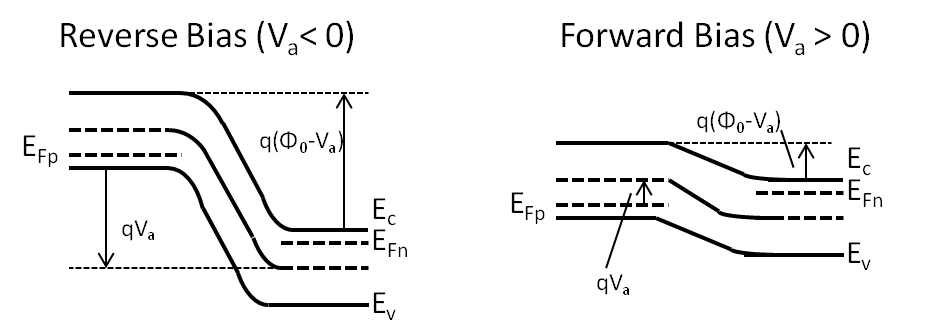
\includegraphics[height=3.5cm,width=8.5cm]{figs/bias_pn_junction}
    \caption{Energy band diagram on $p$-$n$ junction at forward and reverse bias.}
\end{figure}

\section{Current-Voltage Characteristics}\label{sec:cv_ideal}
Thus far ideal $p$-$n$ junctions have been discussed and several assumptions have been made to make 
this possible. First, an abrupt depletion layer has been assumed. This implies that the built-in potential
and applied voltages are supported by a dipole layer with abrupt boundaries, and outside the boundaries the semicondutor is assumed 
to be charge neutral. Second, the Boltzmann approximation has been assumed to be valid. Meaning that the semiconductor
doping level are non-degenerate. If this is not the case then Fermi-Dirac statistics must be employed. 
Third, it has been assumed that the injected minority carrier densities are small compared to the major carrier
densities. If this is not the case, then the high-injection regime has been entered. This will be discussed in more detail in the next section.
Lastly, it is assumed that there is no generation or recombination current present inside the depletion layer,
and the electron and hole currents are constant throughout the depletion layer. Taking these four assumptions into 
account, then the ideal current-voltage characteristics are presented in fig. \ref{fig:fig07}. Note that the minority carriers
are small compared to the majority carriers on each side. The hole current density $J_p$ is large compared to the electron 
carrier density $J_n$ on the $p$-side and the electron carrier density is large compared to the hole carrier density on the $n$-side. In addition,
throughout the depletion region both $J_p$ and $J_n$ are constant in both forward and reverse bias.
\begin{figure}[h!]\label{fig:fig07}
    \centering
    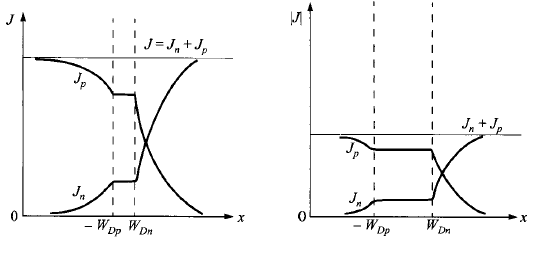
\includegraphics[height=4cm,width=8cm]{figs/schokley_current_reverse_forward}
    \caption{Shockley current density as a function of position within the semiconductor structure at forward and reverse bias.}
\end{figure}

\section{Non-Ideal Current-Voltage Characteristics}
In the previous section the assumptions made for ideal $p$-$n$ junctions was discussed. However,
in reality, $p$-$n$ junctions are from ideal and subject to a number effects in which the aforementioned assumptions
do not hold. Here, two of possible departures will be discussed, as there are many possible effects that could be mentioned, but many
are beyond the scope of this paper. In section \ref{sec:cv_ideal} it was stated that the minority carriers are assumed to be much less than the
majority carriers. First, consider the low-injection regime, where the minority carriers are much less than the majority carriers. In this case
the vast majority of the potential drop occurs across the junction. The hole-concentration in the $n$-side is small compared to the electron concentration
as pictured in the left side of fig. \ref{fig:fig010} and vice versa on the $p$-side. As the high-injection regime approaches, the electron
concentration near the junction increases in order to maintain charge neutrality. If the concentration is increased sufficiently to reach the high-injection regime
as show in the right side of fig. \ref{fig010} then the potential drop across the junction is insignificant compared to the ohmic drops on both sides of the 
neutral regions. 
\begin{figure}[h!]\label{fig:fig010}
    \centering
    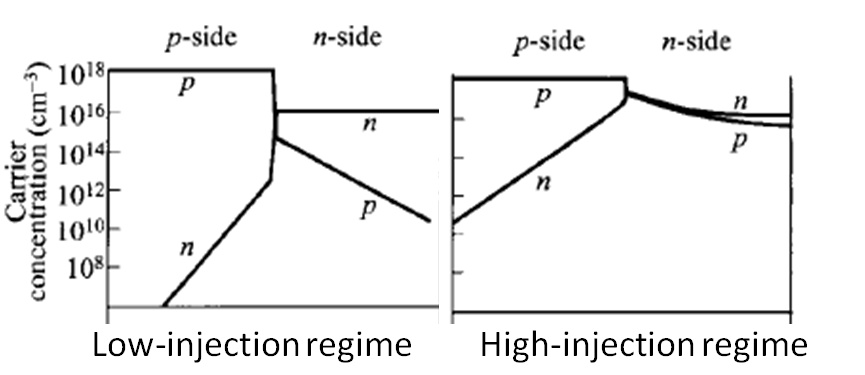
\includegraphics[height=4cm,width=8cm]{figs/high_low_injection}
    \caption{Low and high-injection regimes depicted through carrier densities.}
\end{figure}
Another assumption made in section \ref{sec:cv_ideal} was that generation and recombination does not occur in the depletion 
layer. However, in non-ideal cases, this does occur. Whenever the equilibrium condition of a system is disturbed processes exist to restore
the system to equilibrium. When an external bias is applied, the product $pn$ in the transition region is different from the its equilibrium value
$n_i^2$, since carriers are injected into ($V_a>0$) or extracted from ($V_a<0$) the transition region. 
To restore equilibrium, generation and recombination occurs inside the junction (recombination occurs when $np > n_i^2$ and generation occurs when $np < n_i^2$).
There are two main mechanisms that can occurs in the depletion layer. First, band-to-band recomnbination. This occurs when an electron
moves from its conduction band state into the empty valence band state associated with its hole. This band-to-band transition is also a radiative transition in direct
bandgap semiconductors. A second mechanism is called Schockley-Read Hall (SRH) recombination, also known as trap-assisted recombination.
This occurs when an electron falls into a trap, an energy level within the bandgap caused by some defect. Once the trap is filled it cannot accept another electron.
The electron occupying the trap, in a second step, moves into an empty valence band state, thereby completing the recombination process. This can be envisioned
as a two-step transition of an electron from the conduction band to the valence band or as the annihilation of the electron and the hole, which meet each other in the trap.
The localized state in the gap in can absorb the difference in momentum between the carriers, and so this process is dominant
in indirect bandgap semiconductors, though it can also dominate in direct bandgap material under condtions of very low 
carrier denisities. 

